\pdfinfo{%
  /Title    ()
  /Author   ()
  /Creator  ()
  /Producer ()
  /Subject  ()
  /Keywords ()
}

\section{Gästebucheinträge freischalten}
Hier kann man von Usern verfasste Gästebucheinträge lesen und freischalten. Auf einen Blick erhält man Informationen über den User, der diesen Verfasst hat und den textuellen Inhalt des Gästebucheintrags.
Durch ``Absenden'' kann man die, über Checkboxen ausgewählten Einträge, freischalten. Wählt man ``Zurücksetzen'' aus, dann werden die ausgewählten Checkboxen als nicht ausgwählt markiert.\\
Im unteren Bereich der Anzeige kann man auch direkt zu den anderen Punkten der Admin-Verwaltung springen.\\
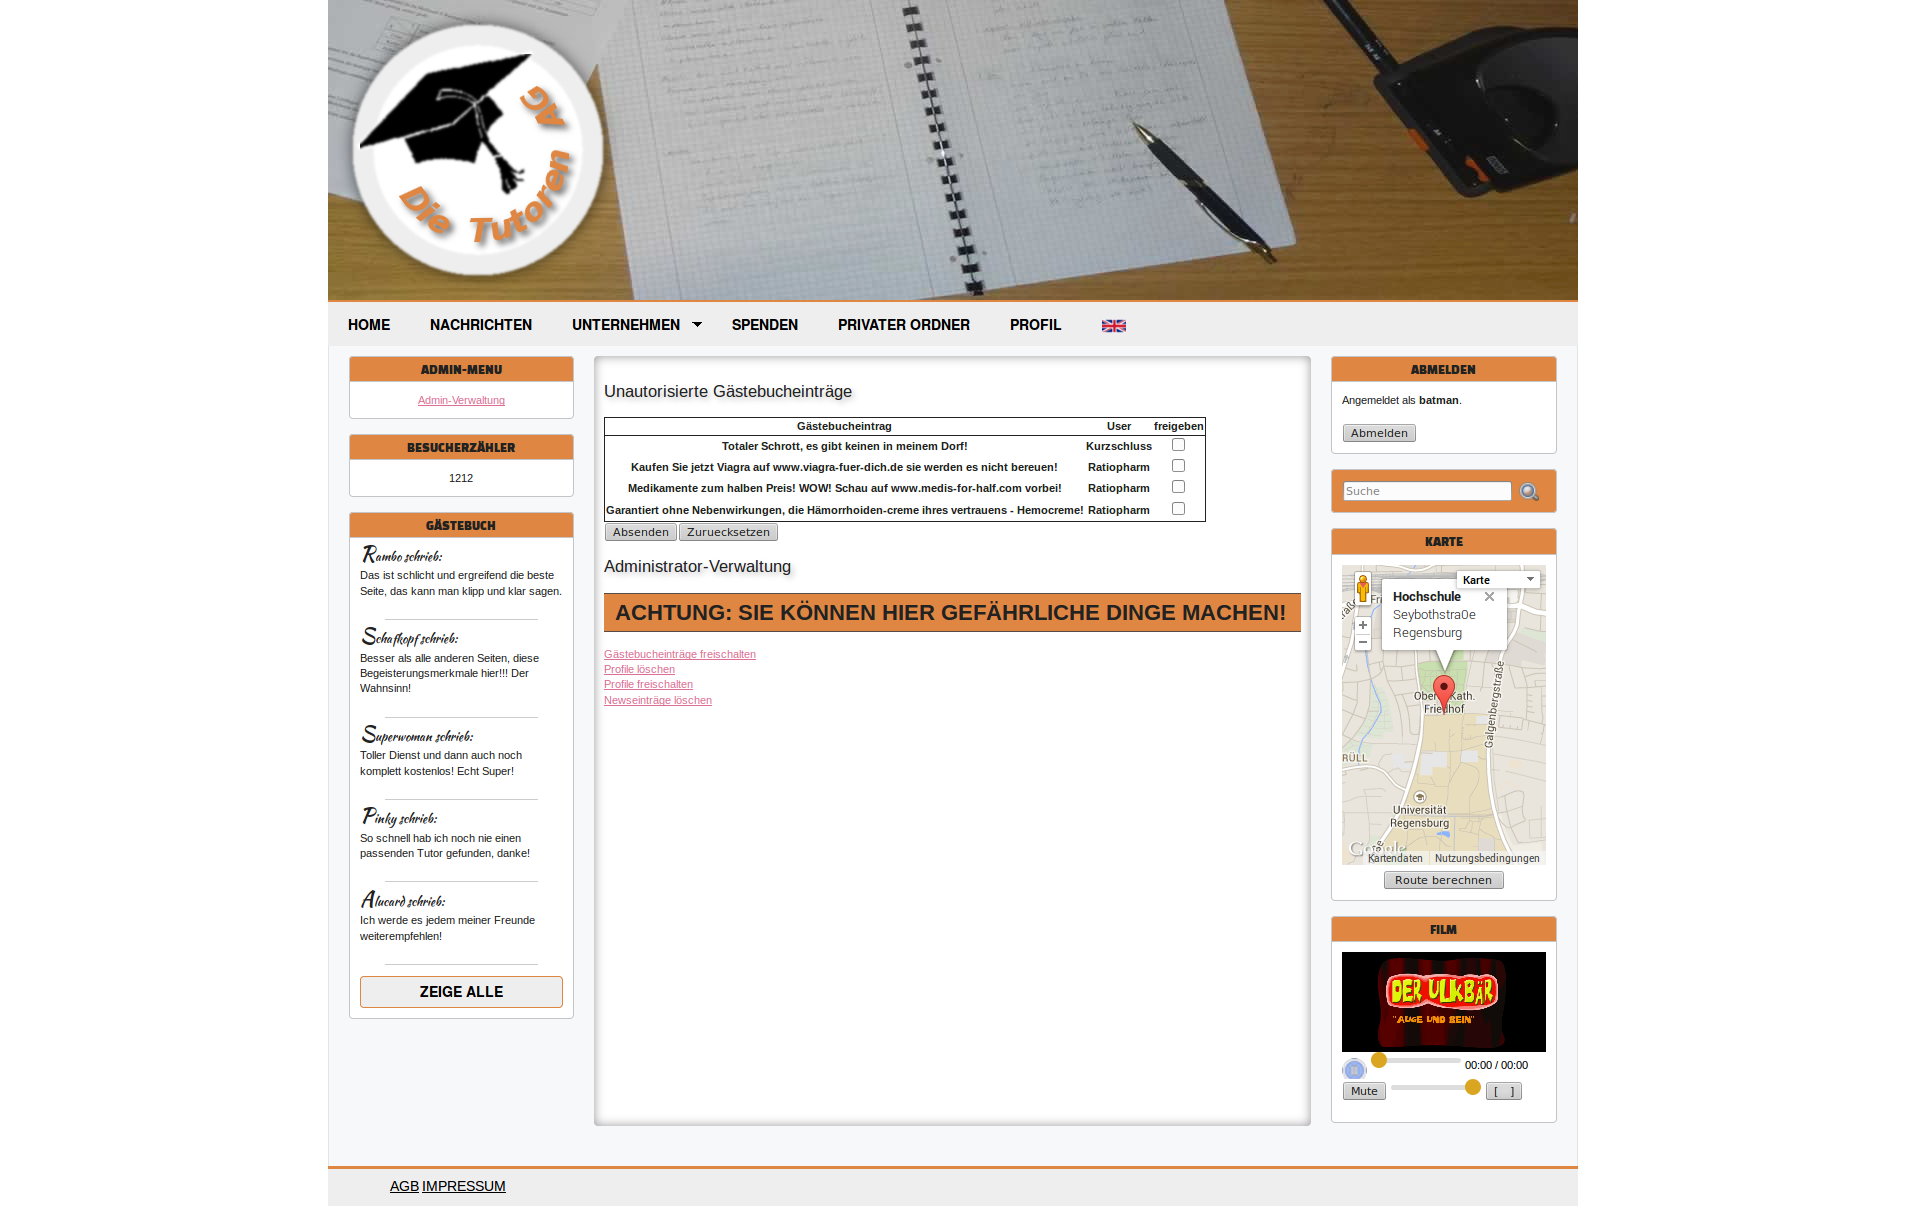
\includegraphics[width=1\textwidth]{../Screenshots/de/admin/admin_guestbook}
